%==============================================================================
% @author Clinton Freeman <freeman@cs.unc.edu>
% @date 2014-05-23
%==============================================================================

\FloatBarrier
\section{Case Study: Melkman's Algorithm}

The DDAD workbench makes it easy for presenters and implementers to quickly
visualize new geometric objects and algorithms. In this section, we overview
using the workbench to implement a bare-bones visualization of Melkman's convex
hull algorithm~\cite{melkman1987line}. First, we implement the basic data
types used by the algorithm and augment their methods with visualization
code. Second, we use these data types to implement Melkman's algorithm. 
By visualizing the data types in an object-oriented way, we arrive at a
clean implementation of the algorithm.

% This section examines using our workbench to animate Melkman's convex hull
% algorithm~\cite{melkman1987line}. 

%==============================================================================

\subsection{Algorithm Overview}

A \emph{polyline} $P$ is a polygonal chain of vertices $p_1, p_2, \ldots, p_n$
connected by line segments $p_ip_{i+1}$ for $1 \leq i < n$. $P$ is \emph{simple}
if the only intersection between segments is at their shared endpoints.
Melkman's algorithm incrementally computes the convex hull of a simple polyline
in $O(n)$ time. 

The algorithm stores the hull's vertices in a doubly-ended queue (deque) and
maintains the invariant that they are stored in ccw order from head to tail,
starting and ending with the most recent vertex added to the hull. The algorithm
establishes the invariant initially by forming the deque with $p_2, p_1, p_2$ to
represent the convex hull of the first two points. 

Now, suppose we wish to add $p_i$ to the hull. Let $v, w$ be the vertices at the
tail of the deque and $u, v$ be the vertices at the head. Thus, $v$ is the most
recent vertex added to the hull, and we can speak of edges $uv$ and $vw$ as
being at the head and tail of the deque, respectively. 

If $p_i$ is not left of $uv$ or inside $uv$, then remove edge $uv$ from the
convex hull by popping the head of the deque; continue until $p_i$ is left of
the edge at the head. Similarly, if $p_i$ is not left of $vw$ or inside $vw$,
then remove edge $vw$ from the convex hull by popping the tail of the deque;
continue until $p_i$ is left of the edge at the tail. Finally, push $p_i$ onto
both the head and tail of the deque to restore the invariant.

On the other hand, if $p_i$ is left or inside both $uv$ and $vw$, then we can 
observe that $p_i$ is not on the convex hull: because the polyline from $v$ to
$p_i$ does not cross the polyline from $u$ to $v$ or from $v$ to $w$, $p_i$ can
leave the hull $CH(P_{i-1})$ only by crossing $uv$ or $vw$. Hull $CH(P_{i-1})$
is identical with $CH(P_i)$, and the invariant already holds.

%==============================================================================

\subsection{Data Type Design and Implementation}

The real work of implementing Melkman's algorithm is designing the data types
upon which it operates. In particular, we require data types for two geometric
objects: input polylines and output polygons. Beyond the standard concerns of
efficiency and ease of use, both data types must support visualization and our
polygon type must support deque semantics.

Our workbench provides an abstract data type, \texttt{Visual::Geometry}, that
geometric data types can inherit to become \emph{visual geometry} types and gain
access to the visualization system. We provide an in-depth discussion of how
\texttt{Visual::Geometry} works in Section~\ref{sec:workbench-architecture}, but
for now it is sufficient to know that uses the observer
pattern~\cite{gamma1994design} to generate and recieve visual events. In
particular, visual geometry objects are able to both observe visual geometry
objects and to be observed by visual geometry objects. A visual geometry object
may \emph{signal} to its observers that a visual event has occurred, and can
optionally implement a \emph{slot} that handles signals from the objects that it
observes. By default, visual geometry objects simply forward signals they
recieve up to their observers, forming an event propagation chain.


A major benefit of visual geometry types is their ability to offload
visualization work through composition. Our polygon type must support deque
operations, but we only require sequential access to the polyline's vertices. In
our case, we can think of the polygon as being composed of a polyline boundary.
This suggests using a deque as a backing store for the polyline's vertices so
that the polygon type may simply delegate deque operations to its boundary. This
choice is consistent with our need for constant sequential access to the
polyline's vertices.



% The \texttt{Polygon\_2r} class is composed of a \text{Polyline\_2r} boundary
% that is responsible for visualizing vertices and edges. It can optionally
% visualize the polygon interior by triangulating it into a fan.  

%  We know from the algorithm description that these should support deque
% semantics, so it makes sense to use this as a backing store for the polygon's
% vertices. In many regards, a polygon will act like a polyline, e.g. we can add
% and remove vertices to both. In order to avoid duplicating functionality, it
% makes sense to compose our polygon with a polyline boundary and forward common
% events to it. We want to visualize both objects, so each will inherit from the
% Visual::Geometry class.

% The \texttt{Polyline\_2r} class uses a deque to store its vertices. The
% \texttt{push\_back} and \texttt{pop\_back} methods are responsible for
% visualizing how those operations affect the visual state of the object.

\lstinputlisting[float,caption=Polyline\_2r
class declaration,label=polyline-class]{code-samples/polyline.cpp}

\lstinputlisting[float,caption=Polygon\_2r
class declaration,label=polygon-class]{code-samples/polygon.cpp}

\lstinputlisting[float,caption=Polyline\_2r
push back
implementation,label=polyline-push-back]{code-samples/polyline-push-back.cpp}
  
%==============================================================================

\FloatBarrier
\subsection{Algorithm Implementation}

Code listing~\ref{melkman-function} shows \texttt{Melkman}, the final C++
implementation of Melkman's algorithm. The function takes as input a
\texttt{Polyline\_2r} and an \texttt{IGeometryObserver}, and produces as output
a \texttt{Polygon\_2r} object. All branching tests make use of the
\texttt{RIsLeftOrInsidePQ} predicate, which encapsulates the logic described in
the previous section.
 
\lstinputlisting[float,caption=Melkman
function implementation,label=melkman-function]{code-samples/melkman.cpp}

%==============================================================================
 
\FloatBarrier
\subsection{Generating Input Data} 



%==============================================================================

% \begin{figure}[h]
% 	\centering
% 	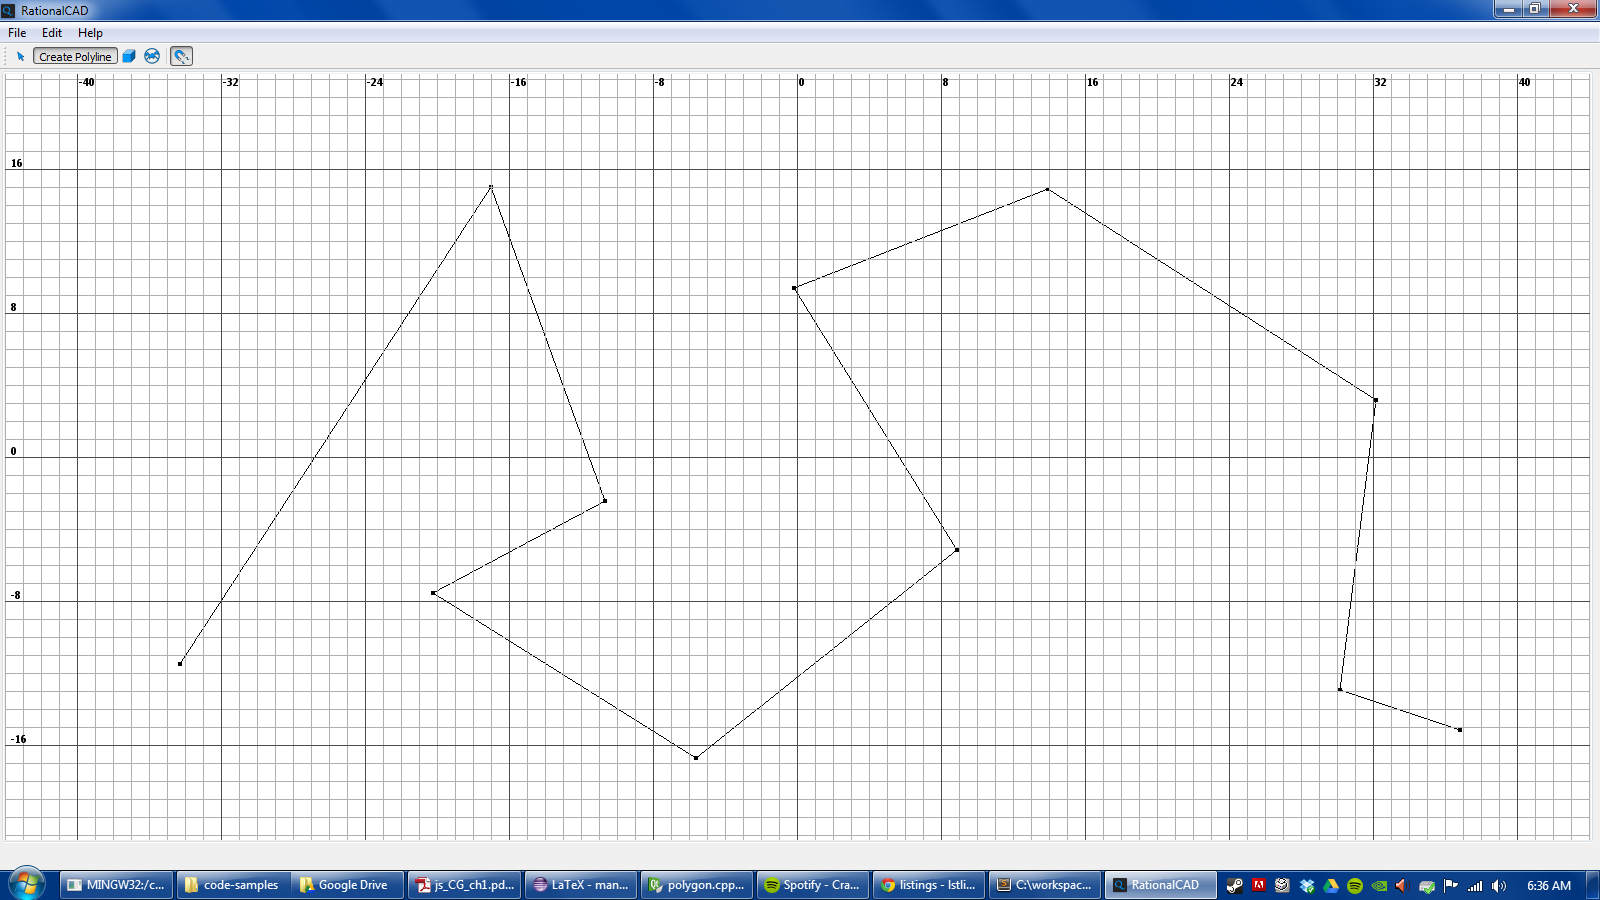
\includegraphics[width=\textwidth]{figures/melkman-input-1}
% 	\caption{Example polyline input.}
% 	\label{fig:melkman-input}
% \end{figure}

 
%As in Figure 1.18,

% Figure 1.19 continues the execution begun in Figure 1.16. It shows all of the
% deques and some of the hulls for $CH(P_5)$ through $CH(P_{14})$. Code is listed
% in Figure 1.20.

% It can also be used to compute the convex
% hull of arbitrary point sets if we first sort by $x$ coordinate, breaking ties
% by $y$ coordinate.

% Melkman's algorithm stores the convex hull vertices in a deque, or doubly-ended
% queue - a simple data structure that stores a list of elements and allows you to
% add and remove (by push() and pop()) elements from the front and back of the
% list. Melkman's algorithm maintains the invariant that the vertices of the
% convex hull CH(P\_i) are stored in a deque in ccw order from head to tail,
% starting and endign with the most recent vertex added to the hull.
% 
% Given an oriented line $pq$ and a point $r$, the 2D orientation predicate
% $\textsc{Orient2D}(p, q, r)$ answers the question, ``is $r$ to the left, right,
% or on $pq$?'' It is often written as the sign of the 2-by-2 determinant, $$
% \textsc{Orient2D}(p, q, r) = \textsc{Sign}\left( \begin{vmatrix} p_x-r_x &
% p_y-r_y \\ q_x-r_x & q_y-r_y \end{vmatrix} \right).$$

% Incremental convex hull algorithms construct the hull by examining each input
% point in turn, exploiting structure in the partial hull to help reduce
% computation. 
% Graham and Yao observed that if we know the points in advance, we
% may make our task easier by considering them in sorted order by $x$ coordinate,
% breaking ties by $y$ coordinate. Then point $p_i$ will always be a vertex of the
% convex hull $\text{CH}(P_i)$, and it will either be adjacent to $p_{i-1}$ or
% will cause $p_{i-1}$ to be removed from $\text{CH}(P_i)$.
 
% \begin{mdframed}[linecolor=white, backgroundcolor=algback, frametitle={Algorithm
% Melkman}] 
% \begin{algorithmic}[1]    
%     \Require Simple polyline $P = \langle v_1, \ldots, v_m \rangle$.
%     \Ensure $\text{CH}(P)$.
%     \vspace{0.75em}
%     \Procedure{Melkman}{$P$}
%     \State $H.push\_back(v_2); H.push\_back(v_1); H.push\_back(v_2);$
%     \Comment{Init hull}
%     \For{$i=3\ldots m$}
%     	\If{\textsc{!LeftOrInside}$(H.back(1), H.back(0), v_i)$ or
%     	\textsc{!LeftOrInside}$(v_i, H.front(1), H.front(0))$} 
%     		\While{\textsc{!LeftOrInside}$(H.back(1), H.back(0), v_i)$}
%     			\State $H.pop\_back();$
%     		\EndWhile
%     		\While{\textsc{!LeftOrInside}$(v_i, H.front(1), H.front(0))$}
%     			\State $H.pop\_front();$
%     		\EndWhile
%     		\State $H.push\_back(v_i);$
%     		\State $H.push\_front(v_i);$
%     	\EndIf
%     \EndFor
%     \State \Return $H$
%     \EndProcedure
% \end{algorithmic}
% \end{mdframed} 

% Animating an algorithm using the workbench is composed of a number of tasks,
% namely 
% \begin{itemize}
%   \item Implement input data structures and instrument them with visualization
%   code.
%   \item Optionally modify the GUI to allow the user to create instances of
%   the input data structure.
%   \item Implement output data structures and instrument them with visualization
%   code.
%   \item Implement predicates.
%   \item Implement the algorithm and instrument it with a small amount of
%   visualization code.
%   \item Optionally modify the GUI to allow the user to run the algorithm on
%   selected input data. 
% \end{itemize}

% \subsection{Data Structures}
% 
% polychain\_2r
% 
% polygon\_2r

% Animating any algorithm begins with generating the appropriate input. In the
% case of Melkman's algorithm, we begin by creating a simple polyline. This is
% accomplished by the user clicking on points in the 2D top-down orthographic
% view. The user may choose to place integer vertex coordinates or turn off
% snapping so that vertex coords are floating point or rational coords.
% 
% 
% 
% \begin{lstlisting}
% Polygon_2r Melkman(const PolyChain_2r& P, Visual::IGeometryObserver* ge_obs) {
%     Polygon_2r CH_P;
% 
% 
%     return CH_P;
% }
% \end{lstlisting}